
%---------------------------------------------
%	6. Application & Perform of GNN Algorithm
%---------------------------------------------

%WIt allowed us to generate realistic data emulating a full Silicon LHC detector (see Fig 3), while providing us with the ground truth of particle trajectory membership. Thus, for each event we obtained the... and, as ground truth, the list of points associated to each track. There is a one to one relationship between the true 3D points and the reconstructed ones.

\chapter{Implementation of the GNN Algorithm to the TrackML Model}
\label{chapter-6}

The following chapter focuses on the implementation of the GNN pattern recognition algorithm to the publicly available dataset designed for the Kaggle TrackML challenge \cite{kaggle-trackml}. The TrackML detector emulates a full silicon LHC detector and as such, certain models of the GNN algorithm outlined in Chapter \ref{chapter-5}, are improved for the TrackML detector geometry.

This chapter is organised as follows. Section \ref{chapter-6-data-prep} describes the structure of the TrackML data and how it was used to build a graph network. Sections \ref{constructing-track-states} and \ref{chapter-6-covariance-derivation} describe the construction of track state estimates. Section \ref{chapter-6-kl-threshold} presents the classifier constructed to determine the optimal KL threshold used within the GMR stage and Section \ref{chapter-6-extrapolation} presents alterations to the extrapolation models used within the Information Aggregation stage. Finally, Section \ref{gnn-kf-implementation} describes specific implementation of KFs used within the state extrapolation as well as within the track fitting stage. 
 





\section{Data Preparation}
\label{chapter-6-data-prep}

The TrackML dataset \cite{kaggle-trackml-data} comprises of multiple independent events, where each event contains simulated measurements (3D points) of particles generated in a collision between proton bunches at the LHC. The training dataset contains the recorded hits and the measured $(x, y, z)$ position of each corresponding hit in the global coordinate system. The event truth data contains each hit's ground truth counterpart, their association to particles and the initial parameters of those particles. The radius at a given point on the particle's trajectory, $r$, is computed using the square root of the sum in quadrature of the global $x$ and $y$ measurements.

In order to read the TrackML data, Python scripts provided by the Kaggle competition organisers are used \cite{python-scripts-kaggle}. The TrackML data provide hit information only, such that graph nodes and edges must be created independently. The hits are converted into graph nodes and edge pairs were constructed using the \textit{FASTrack} algorithm used during the throughput phase of the TrackML Kaggle competition \cite{Amrouche2023}. The FASTrack algorithm is based on a similar hit-pair predictor methodology outlined in Chapter \ref{chapter-4}, whereby hit cluster shapes are used to predict the intervals of track inclination angles and save CPU time by avoiding hit combinations with parameters incompatible with the prediction. Graph edges are predicted and can span up to two layers apart.

Due to the sheer volume of data generated during high-energy proton-proton collisions, it is impossible for any Trigger system to reconstruct all objects. There are many low momentum tracks that will produce hits and will begin to curve under the influence of the magnetic field. These types of tracks are not of interest for reconstruction within this study. As a result, there are certain kinematic requirements imposed. Constraints are embedded on the graph edge parameters, in order to select the tracks of interest with a particular $p_{\text{T}}$ from the very beginning \cite{Dmitry-fasttrack-addtest}, and construct the graph network. 

% min_Curvature - want to select a particular pT range of the tracks we want to look at
% repo - "fasttrack" add-test branch


\section{Construction of Track State Estimates}
\label{constructing-track-states}

Track state estimates, $X_{ij}$, are constructed using a parabolic model for parameters in the transverse $x$-$y$ plane and a linear model for parameters in the $r$-$z$ plane.

% In order to construct track state estimates, $X_{ij}$, for each connection between node $i$ and its neighbour $j$, track parameters in both the transverse $x$-$y$ plane and the $r$-$z$ plane are considered.


\subsection{Parabolic Track Model}
\label{parabolic-state}

In the $x$-$y$ plane, charged particles experience the influence of the magnetic field and their trajectories follow a near-parabolic shape. As illustrated in Figure \ref{fig:gnn-parabolic-model}, a parabola is formed using the global origin O, node A and neighbour node B. The parabola is transformed into the local coordinate system of node A such that the new $x$-axis, $X_A$, is parallel to O - A and the new $y$-axis, $Y_A$, is the perpendicular. 

\begin{figure}[htbp!] 
    \centering
    \subfloat[]{%
        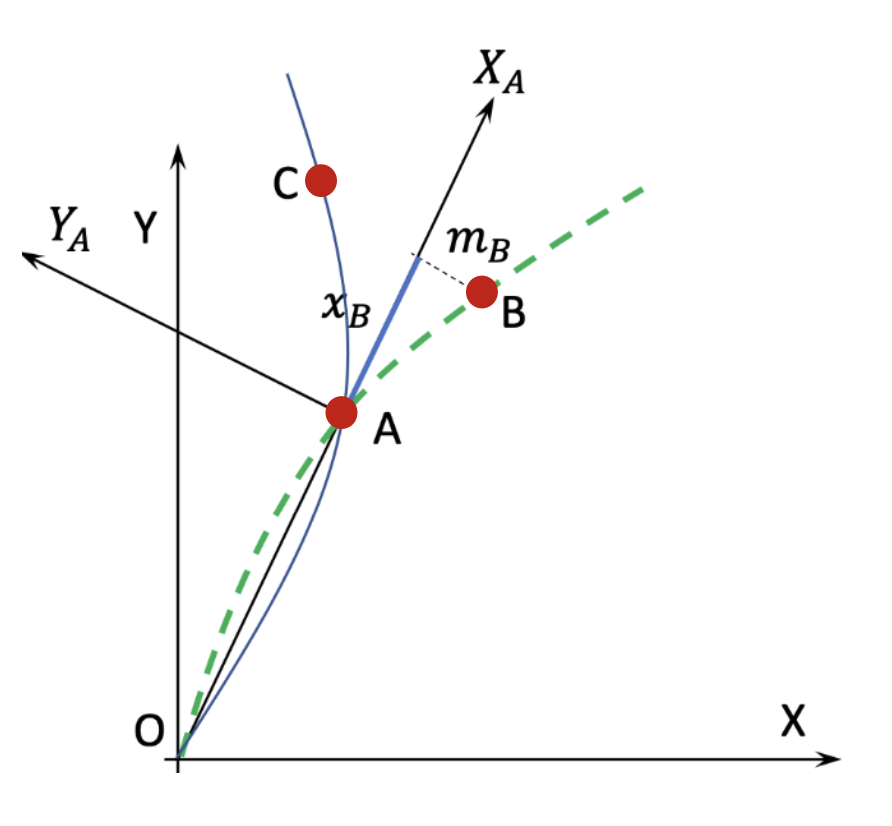
\includegraphics[width=0.42\textwidth]{images/5-gnn-algorithm/parabolic-state-model-1.png}%
        \label{fig:gnn-parabolic-state-1}%
        }%
    \hfill%
    \subfloat[]{%
        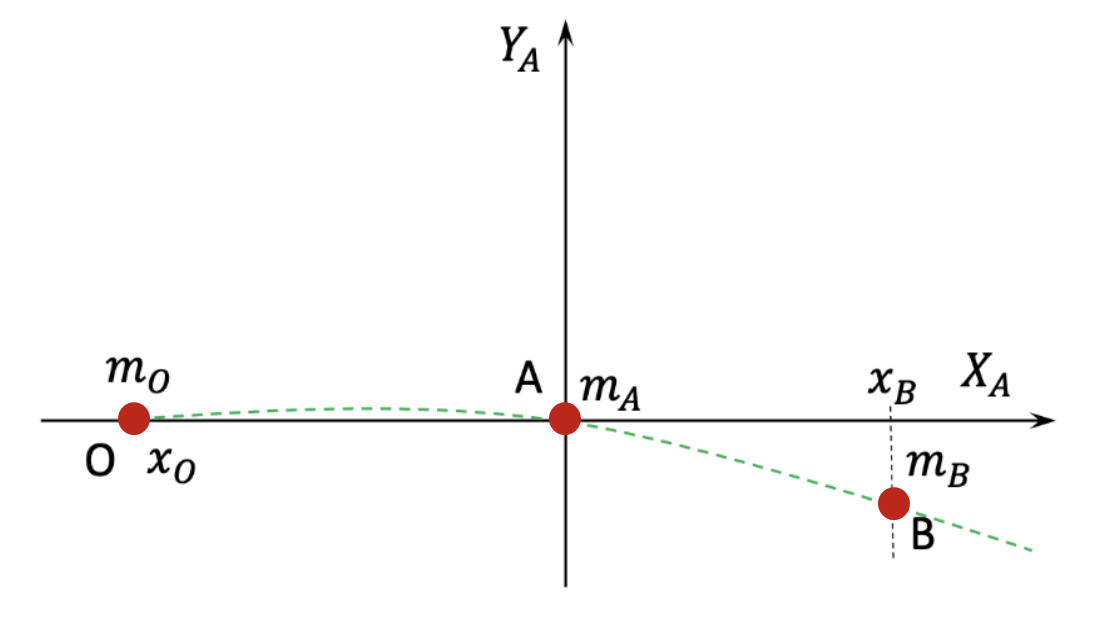
\includegraphics[width=0.56\textwidth]{images/5-gnn-algorithm/parabolic-state-model-2.png}%
        \label{fig:gnn-parabolic-state-2}%
        }%
    \caption{Parabolic model illustration. a) Construction of example parabolas O - A - B and O - A - C, where O is the global origin and A, B, C are graph nodes. b) Rotation of parabola O - A - B into the local coordinate system of A.}
    \label{fig:gnn-parabolic-model}
\end{figure}


Using the quadratic equation of a parabola, the vector of measurements in the local coordinate system of node A, $ \hat{m} = [m_O \quad m_A \quad m_B]^{T}$ can be expressed in terms of the unknown parabolic coefficients $\hat{p} = [a \quad b \quad c]^{T}$ using Eq \eqref{eqn:parabolic-equations}, 

\begin{equation}
    \hat{m} = H_{xy} \hat{p} 
    \label{eqn:parabolic-equations}
\end{equation}

where $m_O$, $m_A$ and $m_B$ are the respective measurements of the global origin O, node A and node B, transformed into the local coordinate system of node A, and $\{a, b, c\}$ are the parabolic coefficients. Measurements $m_O = 0$ and $m_A = 0$, as illustrated in Figure \ref{fig:gnn-parabolic-state-2}. The measurement matrix, $H_{xy}$, relates the measurement vector $\hat{m}$, to the vector of parabolic parameters $\hat{p}$ and is given by Eq \eqref{eqn:trackml-matrix-h-xy},

\begin{equation}
    H_{xy} = \begin{bmatrix} x_O^{2} & x_O & 1 \\ 0 & 0 & 1 \\ x_B^{2} & x_B & 1 \end{bmatrix} 
    \label{eqn:trackml-matrix-h-xy}
\end{equation}

where $x_O$ and $x_B$ are the $x$-coordinates of global origin O and node B in the local coordinate system of node A. The parabolic parameters are derived using Eq \eqref{eqn:derive-p}.

\begin{equation}
    \hat{p} = H_{xy}^{-1} \hat{m} 
    \label{eqn:derive-p}
\end{equation}


% \begin{equation}
% \begin{aligned}
% m_O = ax_{O}^{2} + bx_O + c \\
% m_A = c \\
% m_B = ax_{B}^{2} + bx_B + c
% \end{aligned}
% \label{eqn:parabolic-equations}
% \end{equation}


\subsection{Linear Track Model}
\label{linear-state}

The $r$-$z$ plane is parallel to the direction of travel of the beamline, where tracks follow a linear model. The inverse track inclination, $\tau$, between node A and neighbour B, is given by Eq \eqref{eqn:tau-parameter}, where $(z_A, r_A)$ refer to measurements of node A and $(z_B, r_B)$ refer to measurements of neighbour node B.

\begin{equation}
\tau = \frac{z_A - z_B}{r_A - r_B}
\label{eqn:tau-parameter}
\end{equation}

\subsection{Combined Track State Estimate}

Parabolic parameters $\{a, b\}$ derived using Section \ref{parabolic-state}, as well as the inverse track inclination, $\tau$, given in Eq \eqref{eqn:tau-parameter}, provide an indication of track orientation. Hence, the track state estimate, $X_{ij}$, between node $i$ and neighbour $j$ is given by Eq \eqref{eqn:joint-state-vector}.

\begin{equation}
X_{ij} = \begin{bmatrix} a \\ b \\ \tau \end{bmatrix}
\label{eqn:joint-state-vector}
\end{equation}







\section{Derivation of Edge State Covariance}
\label{chapter-6-covariance-derivation}

To derive the edge state covariance, $C_{ij}$, of $X_{ij}$ given by Eq \eqref{eqn:joint-state-vector}, the covariance of the track state parameters in the $x$-$y$ and $r$-$z$ planes are handled separately. 


\subsection{Covariance of Parabolic Parameters}

The joint measurement covariance matrix, $S_{xy}$, for a parabola constructed in the $x$-$y$ plane using the global origin O and nodes A and B, as illustrated in Figure \ref{fig:gnn-parabolic-state-2}, is stated in Eq. \eqref{eqn:trackml-s-matrix-xy}


\begin{equation}
    S_{xy} = \begin{bmatrix} \sigma_O^{2} & 0 & 0 \\ 0 & \sigma_A^{2} & 0 \\ 0 & 0 & \sigma_B^{2} \end{bmatrix} 
    \label{eqn:trackml-s-matrix-xy}
\end{equation}

where $\sigma_O$, $\sigma_A$ and $\sigma_B$ are the respective errors due to the measurements at the global origin O, node A and node B, using the parabolic model approximation outlined in Section \ref{parabolic-state}. The measurement error in the global origin $\sigma_O$ is initialised to 4.0mm due to the large error in the beamspot, whereas $\sigma_A$ and $\sigma_B$ are initialised to 0.3mm due to the high precision of the Pixel detector. Hence, the covariance of the vector of parabolic parameters $\hat{p}$, is given by $C_{xy}$ in Eq \eqref{eqn:c-xy}

\begin{equation}
    C_{xy} = H_{xy}^{-1}S_{xy}{H_{xy}^{-1}}^{T}
    \label{eqn:c-xy}
\end{equation}






\subsection{Variance in Inverse Track Inclination}

The joint measurement covariance matrix, $S_{rz}$, for node $i$ and neighbour node $j$ in the $r$-$z$ plane is stated in Eq \eqref{eqn:trackml-s-matrix-rz}

\begin{equation}
    S_{rz} = \begin{bmatrix} \sigma_{zi}^{2} & 0 & 0 & 0 \\ 
                             0 & \sigma_{zj}^{2} & 0 & 0 \\ 
                             0 & 0 & \sigma_{ri}^{2} & 0 \\
                             0 & 0 & 0 & \sigma_{rj}^{2}
                            \end{bmatrix} 
    \label{eqn:trackml-s-matrix-rz}
\end{equation}


where $\{ \sigma_{zi}, \sigma_{zj} \}$ are the measurement errors along the $z$-axis and $\{ \sigma_{ri}, \sigma_{rj} \}$ are the measurement errors in $r$, for the respective $i$ and $j$ nodes. The error in the track inclination $\tau$ is computed using the standard error propagation and linear algebra approach. The transition Jacobian, $J_{rz}$, relates the measurements in the $r$-$z$ plane to the inverse track inclination $\tau$ and is given by Eq \eqref{trackml-g-rz}.

\begin{equation}
    J_{rz} = \begin{bmatrix} 
            (r_i - r_j)^{-1} &
            -(r_i - r_j)^{-1} & 
            \frac{-(z_i - z_j)}{(r_i - r_j)^2} & 
            \frac{z_i - z_j}{(r_i - r_j)^2}
            \end{bmatrix} 
    \label{trackml-g-rz}
\end{equation}

The corresponding error in track inclination $\tau$ is given by Eq \eqref{eqn:error-in-tau}

\begin{equation}
    \sigma_{\tau} = J_{rz} S_{rz} J_{rz}^{T}
    \label{eqn:error-in-tau}
\end{equation}






\subsection{Moli\`ere Theory of Multiple Scattering}

A charged particle traversing a medium is deflected by many small-angle scatters. Most of this deflection is due to Coulomb scattering from nuclei. However, for hadronic projectiles the strong interactions also contribute to multiple scattering. Therefore, the error in track direction will have a contribution from the observed error due to multiple scattering, $\sigma_{ms}$. The scattering distribution is well represented by the theory of Moli\`ere, which is roughly Gaussian for small deflection angles. The contribution due to Moli\`ere multiple scattering is given by the simplified Highland formula \cite{moliere-theory-formula, Lynch:1990sq} stated in Eq \eqref{eqn:simplified-moliere-equation}.

%The Moli\`ere multiple scattering is inversely proportional to particle full momentum and proportional to the square root of material thickness.

% \begin{equation}
%     \sigma_{ms}^{2} = \frac{13.6 \text{MeV}}{\beta c p} z \sqrt{\frac{x}{X_0}} \left[ 1 + 0.038ln \left( \frac{x}{X_0} \right) \right] 
%     \label{eqn:moliere-equation}
% \end{equation}

\begin{equation}
    \sigma_{ms}^{2} = \frac{13.6 \text{MeV}}{\beta c p} z \sqrt{\frac{x}{X_0}}
    \label{eqn:simplified-moliere-equation}
\end{equation}

where $p$, $\beta c$, and $z$ are the full momentum, velocity, and charge number of the incident particle, and $x/X_0$ is the thickness of the scattering medium, measured in radiation lengths. For simplicity, $\beta c$ and $z$ are set to 1. 




\subsubsection{Derivation of Full Momentum}

The full particle momentum, $p$, is given by Eq \eqref{eqn:full-momentum}

\begin{equation}
    p = p_\text{T} / sin(\theta)
    \label{eqn:full-momentum}
\end{equation}

where $p_\text{T}$ is the transverse momentum of the particle and $\theta$ is the angle of inclination of the particle trajectory to the $z$-axis. The transverse momentum, $p_\text{T}$, for a charged particle in the presence of a magnetic field is given by Eq \eqref{eqn:transverse-momentum}

\begin{equation}
    p_\text{T} = B q r
    \label{eqn:transverse-momentum}
\end{equation}

where $p_\text{T}$ is measured in GeV/c, B is the magnetic field of the TrackML model set to 0.3T, $q$ is the charge of the particle set to 1 and $r$ is the radius of particle's trajectory. The radius $r$ is inversely proportional to the track curvature $\kappa$, given by Eq \eqref{eqn:kappa}, 

\begin{equation}
\kappa = \frac{2a}{(1 + (2ax + b)^2)^{\frac{3}{2}}}
\label{eqn:kappa}
\end{equation}

where $\kappa$ is a function of parabolic parameters $a$ and $b$, and $x$ is the $x$-coordinate of the point at which the curvature is calculated. Therefore, the full momentum $p$ is hence given by Eq \eqref{eqn:full-momentum-derived} using the knowledge that $\kappa = 1/r$.

\begin{equation}
p = B / \kappa sin(\theta)
\label{eqn:full-momentum-derived}
\end{equation}


\subsubsection{Orientation of Detector Layers}

If a particle crosses one of the TrackML detector layers at incident angle $\theta$, then the radiation length is $0.02 f(\theta)$, where 0.02 is the integrated $x/X_0$ for a typical silicon detector layer which is considered as a single thin scatter. $f(\theta)$ is determined by the orientation of the detector layer, depending upon the mutual orientation of the node-pair. For example, for a scattered node in the barrel, the intersected radiation length becomes $0.02 / sin(\theta)$ and for a scattered node in the endcap $0.02 / cos(\theta)$.


\subsubsection{Contribution to Edge State Covariance}

Barrel version of var ms and endcap version of var ms.

contribution of error due to multiple-scattering only affects the track direction - which is reflected in parabolic parameter b, so that's why we only add this contribution to the corresponding b parameter in the matrix and the tau parameter (cov(1,1) and cov(2,2)).


\begin{itemize}
\item how were the edge state covariances dervied and the sigma errors chosen

\end{itemize}


\subsection{Combined Edge State Covariance}

The edge state covariance matrix of the combined track state estimate $X_{ij}$, is given by $C_{ij}$ in Eq \eqref{eqn:combined-edge-state-covariance}.

\begin{equation}
    C_{ij} = \begin{bmatrix} 
            C_{xy}^{00} & C_{xy}^{01} & 0 \\ 
            C_{xy}^{10} & C_{xy}^{11} + \sigma_{ms}^2 & 0 \\ 
            0 & 0 & \sigma_{\tau}^{2} + \sigma_{ms}^2 \\
            \end{bmatrix} 
    \label{eqn:combined-edge-state-covariance}
\end{equation}

where $C_{xy}^{00}$, $C_{xy}^{01}$, $C_{xy}^{10}$ and $C_{xy}^{11}$ are the corresponding matrix components of the covariance of the vector of parabolic parameters $\hat{p}$, $C_{xy}$, in the $x$-$y$ plane, stated in Eq \eqref{eqn:c-xy}, and $\sigma_{\tau}^2$ is the variance of the inverse track inclination $\tau$, stated in Eq \eqref{eqn:error-in-tau}. The combined edge state covariance, $C_{ij}$, is therefore represented as a 2x2 block matrix of the $[cov(a, b)]$ extracted from $C_{xy}$, and the variance in the $\tau$ component.

The non-diagonal elements of $C_{ij}$ in the third dimension are zero as there is no correlation in measurements between the $x$-$y$ and $r$-$z$ plane for the Pixel detector.

Components of $X_{ij}$, that represent the error in track direction must have a contribution from the observed error due to multiple scattering, $\sigma_{ms}$. Therefore, the variance due to multiple scattering, $\sigma_{ms}^2$ must be added to the variance of parameters $b$ and $\tau$, represented by matrix components $C_{ij}^{11}$ and $C_{ij}^{22}$.




\section{The Optimal KL Threshold}
\label{chapter-6-kl-threshold}

During stage 1 of the GNN algorithm, GMR via k-means clustering is used to reduce the Gaussian mixture of states present at each node. In order to establish if track state estimates, $X_{ij}$, can be grouped into a cluster, the KL divergence, $d_{KL}$, is used as a threshold distance as it is a measure of the statistical distance between two Gaussian probability distributions \cite{KL, FRUHWIRTH19971}.

To determine the optimal pairwise $d_{KL}$ between $X_{ij}$ for a given node, a SVM classifier was trained. Pairwise $d_{KL}$ and $\sigma_{e}^{2}$ for a given node are used as input features. A MC simulation of $10,000$ particle collision events, each event with ten truth tracks, was used to build a training dataset. Loosely compatible edge connections were formed using a hit-pair predictor based on track inclination angle of neighbouring hits, similar to the graph network constructed in \ref{fig:heat-map}. The feature vector was comprised of $\sigma_{e}$ for a given node and pairwise $d_{KL}$ between its track states. The truth particle was extracted for each pairwise connection, where truth 1 corresponded to hits from both track states originating from the same truth particle, and truth 0 otherwise. 

%The truth data is presented is Figure \ref{fig:KL-distance-truth}.

A SVM was trained to discriminate between the two classes \cite{scikit-learn}, using a polynomial degree three kernel. SVM predictions were adjusted such that the TPR was tuned to 95\% in order to maintain a high purity. The SVM decision boundary was converted into a fast LUT using a similar methodology outlined in Section \ref{LUT-generation} and was directly used within the k-means clustering of the GMR stage. If $d_{KL}$ $\leq$ the predicted threshold for a node with particle $\sigma_e$, then pairwise states were clustered together and merged into a single state $X^M$.

% The predictions and corresponding decision boundary is shown in Figure \ref{fig:KL-distance-predictions}.

Other classification algorithms were explored, however the SVM was the most appropriate to determine a decision boundary to best separate the classes.

% \begin{figure}[htbp!] 
%     \centering
%     \subfloat[Ground truth data from MC simulation]{%
%         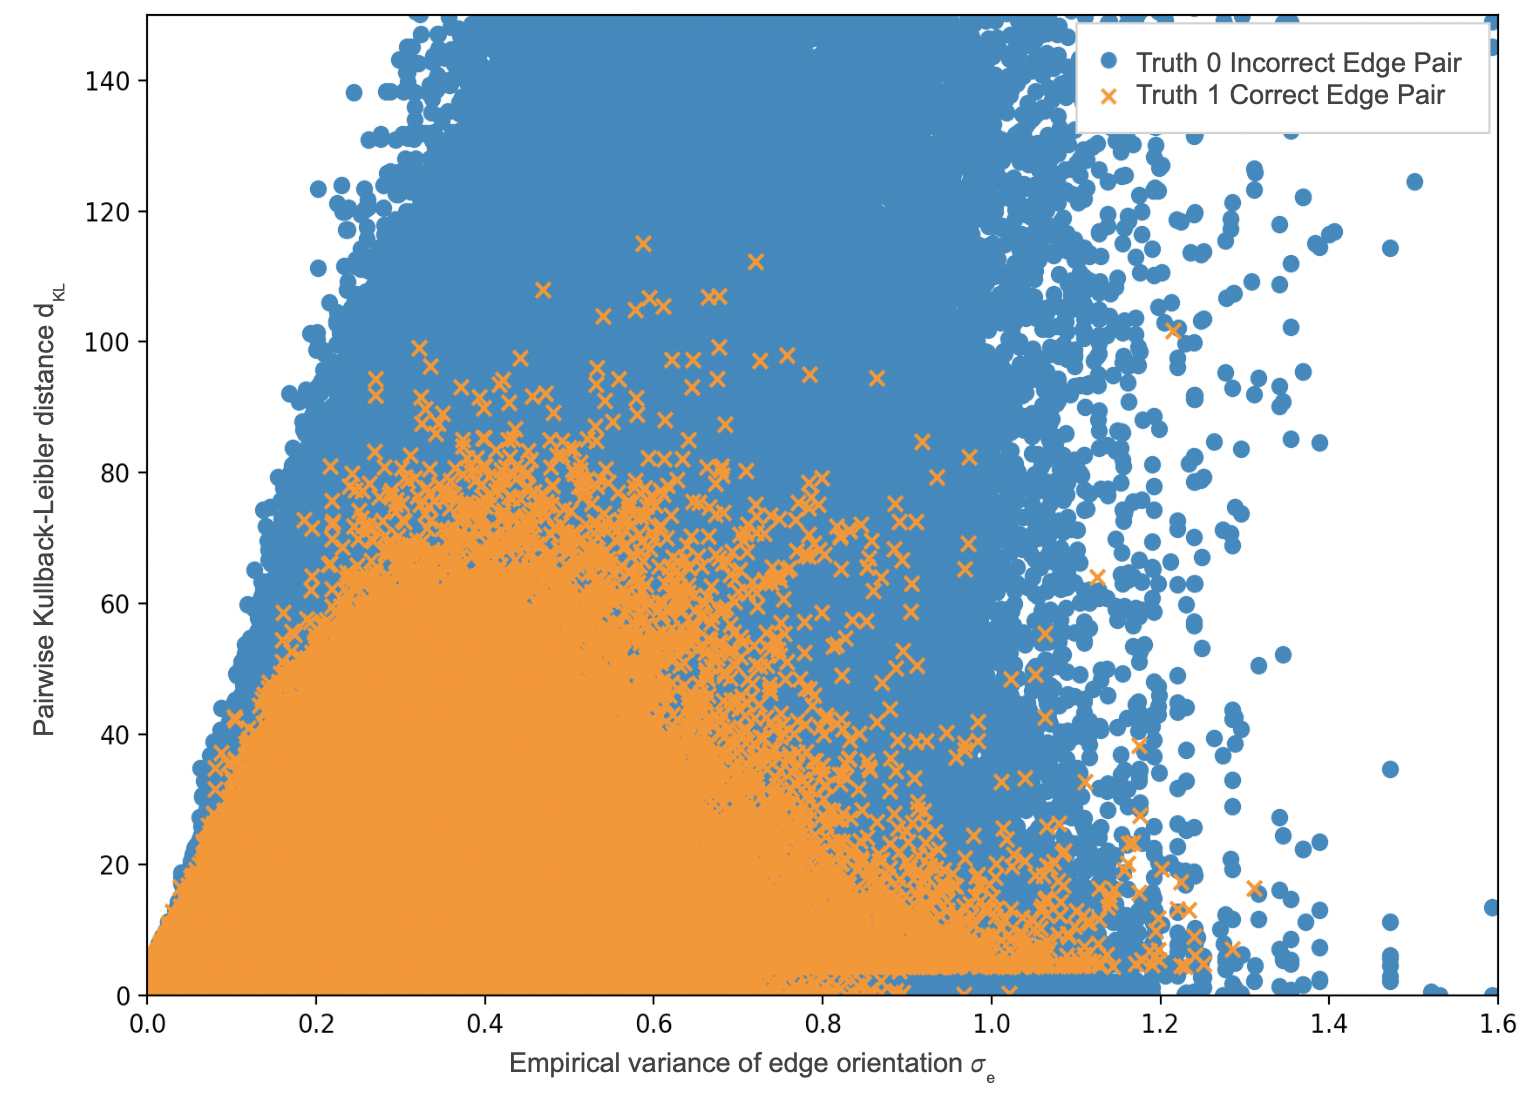
\includegraphics[width=0.85\linewidth]{images/6-results/kl-truth.png}%
%         \label{fig:KL-distance-truth}%
%         }%
%     \hfill%
%     \subfloat[SVM predictions and decision boundary]{%
%         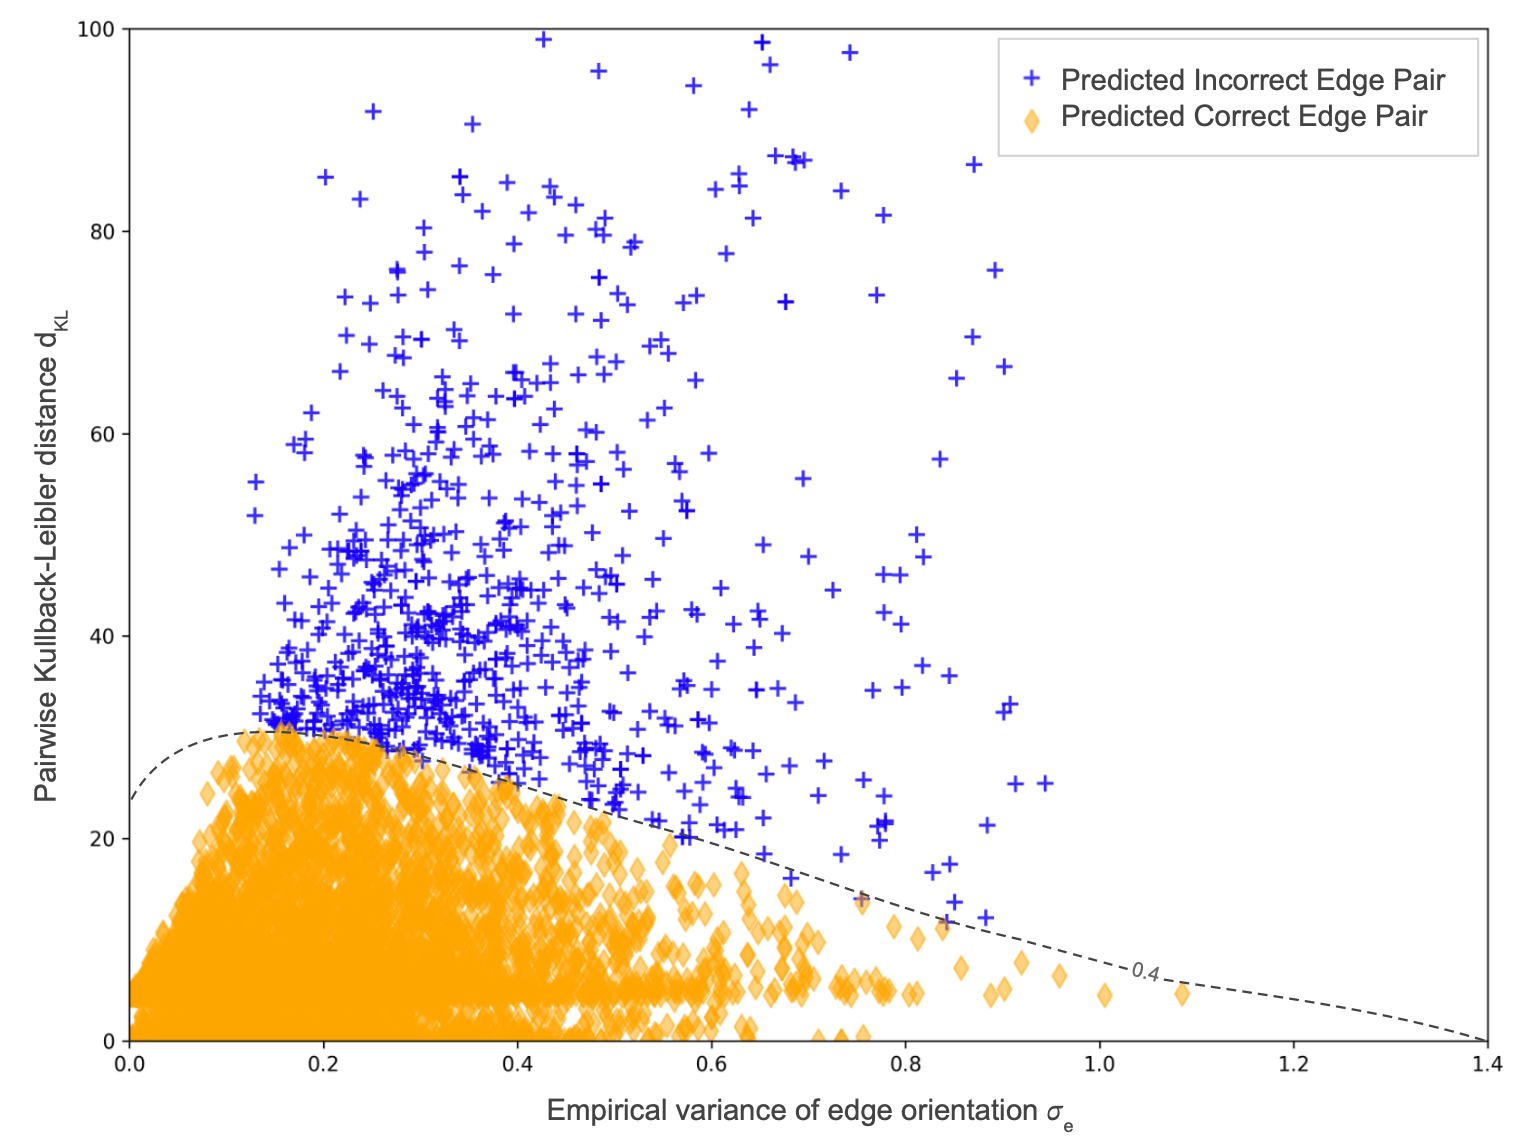
\includegraphics[width=0.85\linewidth]{images/6-results/kl-predictions.png}%
%         \label{fig:KL-distance-predictions}%
%         }%
%     \caption{........}
%     \label{fig:KL-distance}
% \end{figure}





\section{Extrapolation Models}
\label{chapter-6-extrapolation}

\subsection{Parabolic Extrapolation Model}
\begin{itemize}
    \item Information propagation via Message Passing Mechanism
    \item Extrapolation and Validation
    \item Linear and Parabolic model - 2 different extrapolations for xy componenets of state vector and rz componenet, illustrations here
    \item Kalman Filter Update, OU process for correlated noise
\end{itemize}

Mention here that both the linear and parabolic models were used in this instance, where the track state estimate comprised of a 3x1 vector, a, b, tau. The extrapolation and KF update will be different here, different transition Jacobian matrix. Also mention about tuning the chi2 distance thresholds during extrapolation

%The matrix $\widetilde{C}_{ij}$ includes the addition of the process noise $Q$ modelled by the Ornstein-Uhlenbeck (OU) process \cite{OU} which encompasses all material effects. See Section \ref{kf} for further details. The full derivation of $F$ and $Q$ are shown in Appendix \ref{appendix:Appendix-A}

\subsection{Linear Extrapolation Model}


\section{Implementation of Kalman Filters}
\label{gnn-kf-implementation}

\subsection{KF for Extrapolation}
Mention about the OU process noise, for correlated noise etc, 
2 different KFs here - 1 for rz linear extrapolation and 1 for xy

\subsection{KF for Track Fitting}
2 different KFs here - 1 for rz track fit and 1 for xy track fit

%\begin{itemize}
%\item emphasis on the use of KFs both in information aggregation stage and in track extraction, both are implemented in different ways, is a useful and unique part to this algorithm
%\item OU process noise
%\end{itemize}

